%-----------------------------------------------------------------------------%
\chapter{\babEmpat}
%-----------------------------------------------------------------------------%

Bab ini menyajikan hasil eksperimen dari implementasi sistem deteksi \textit{deepfake} menggunakan \textit{ensemble weighted averaging} yang menggabungkan empat arsitektur \textit{deep learning}. Hasil yang disajikan meliputi analisis performa model individual, implementasi sistem \textit{ensemble}, evaluasi komparatif, dan diskusi komprehensif terhadap \textit{findings} yang diperoleh.

%-----------------------------------------------------------------------------%
\section{Overview Pipeline Eksperimen}
%-----------------------------------------------------------------------------%

Sebelum menyajikan hasil detail, penting untuk memahami keseluruhan pipeline implementasi yang telah dilakukan. Gambar~\ref{fig:implementation_pipeline} mengilustrasikan tahapan lengkap eksperimen, mulai dari pre-processing hingga post-processing, yang menjadi dasar bagi semua hasil yang akan dibahas dalam bab ini.

\begin{figure}[H]
    \centering
    \fbox{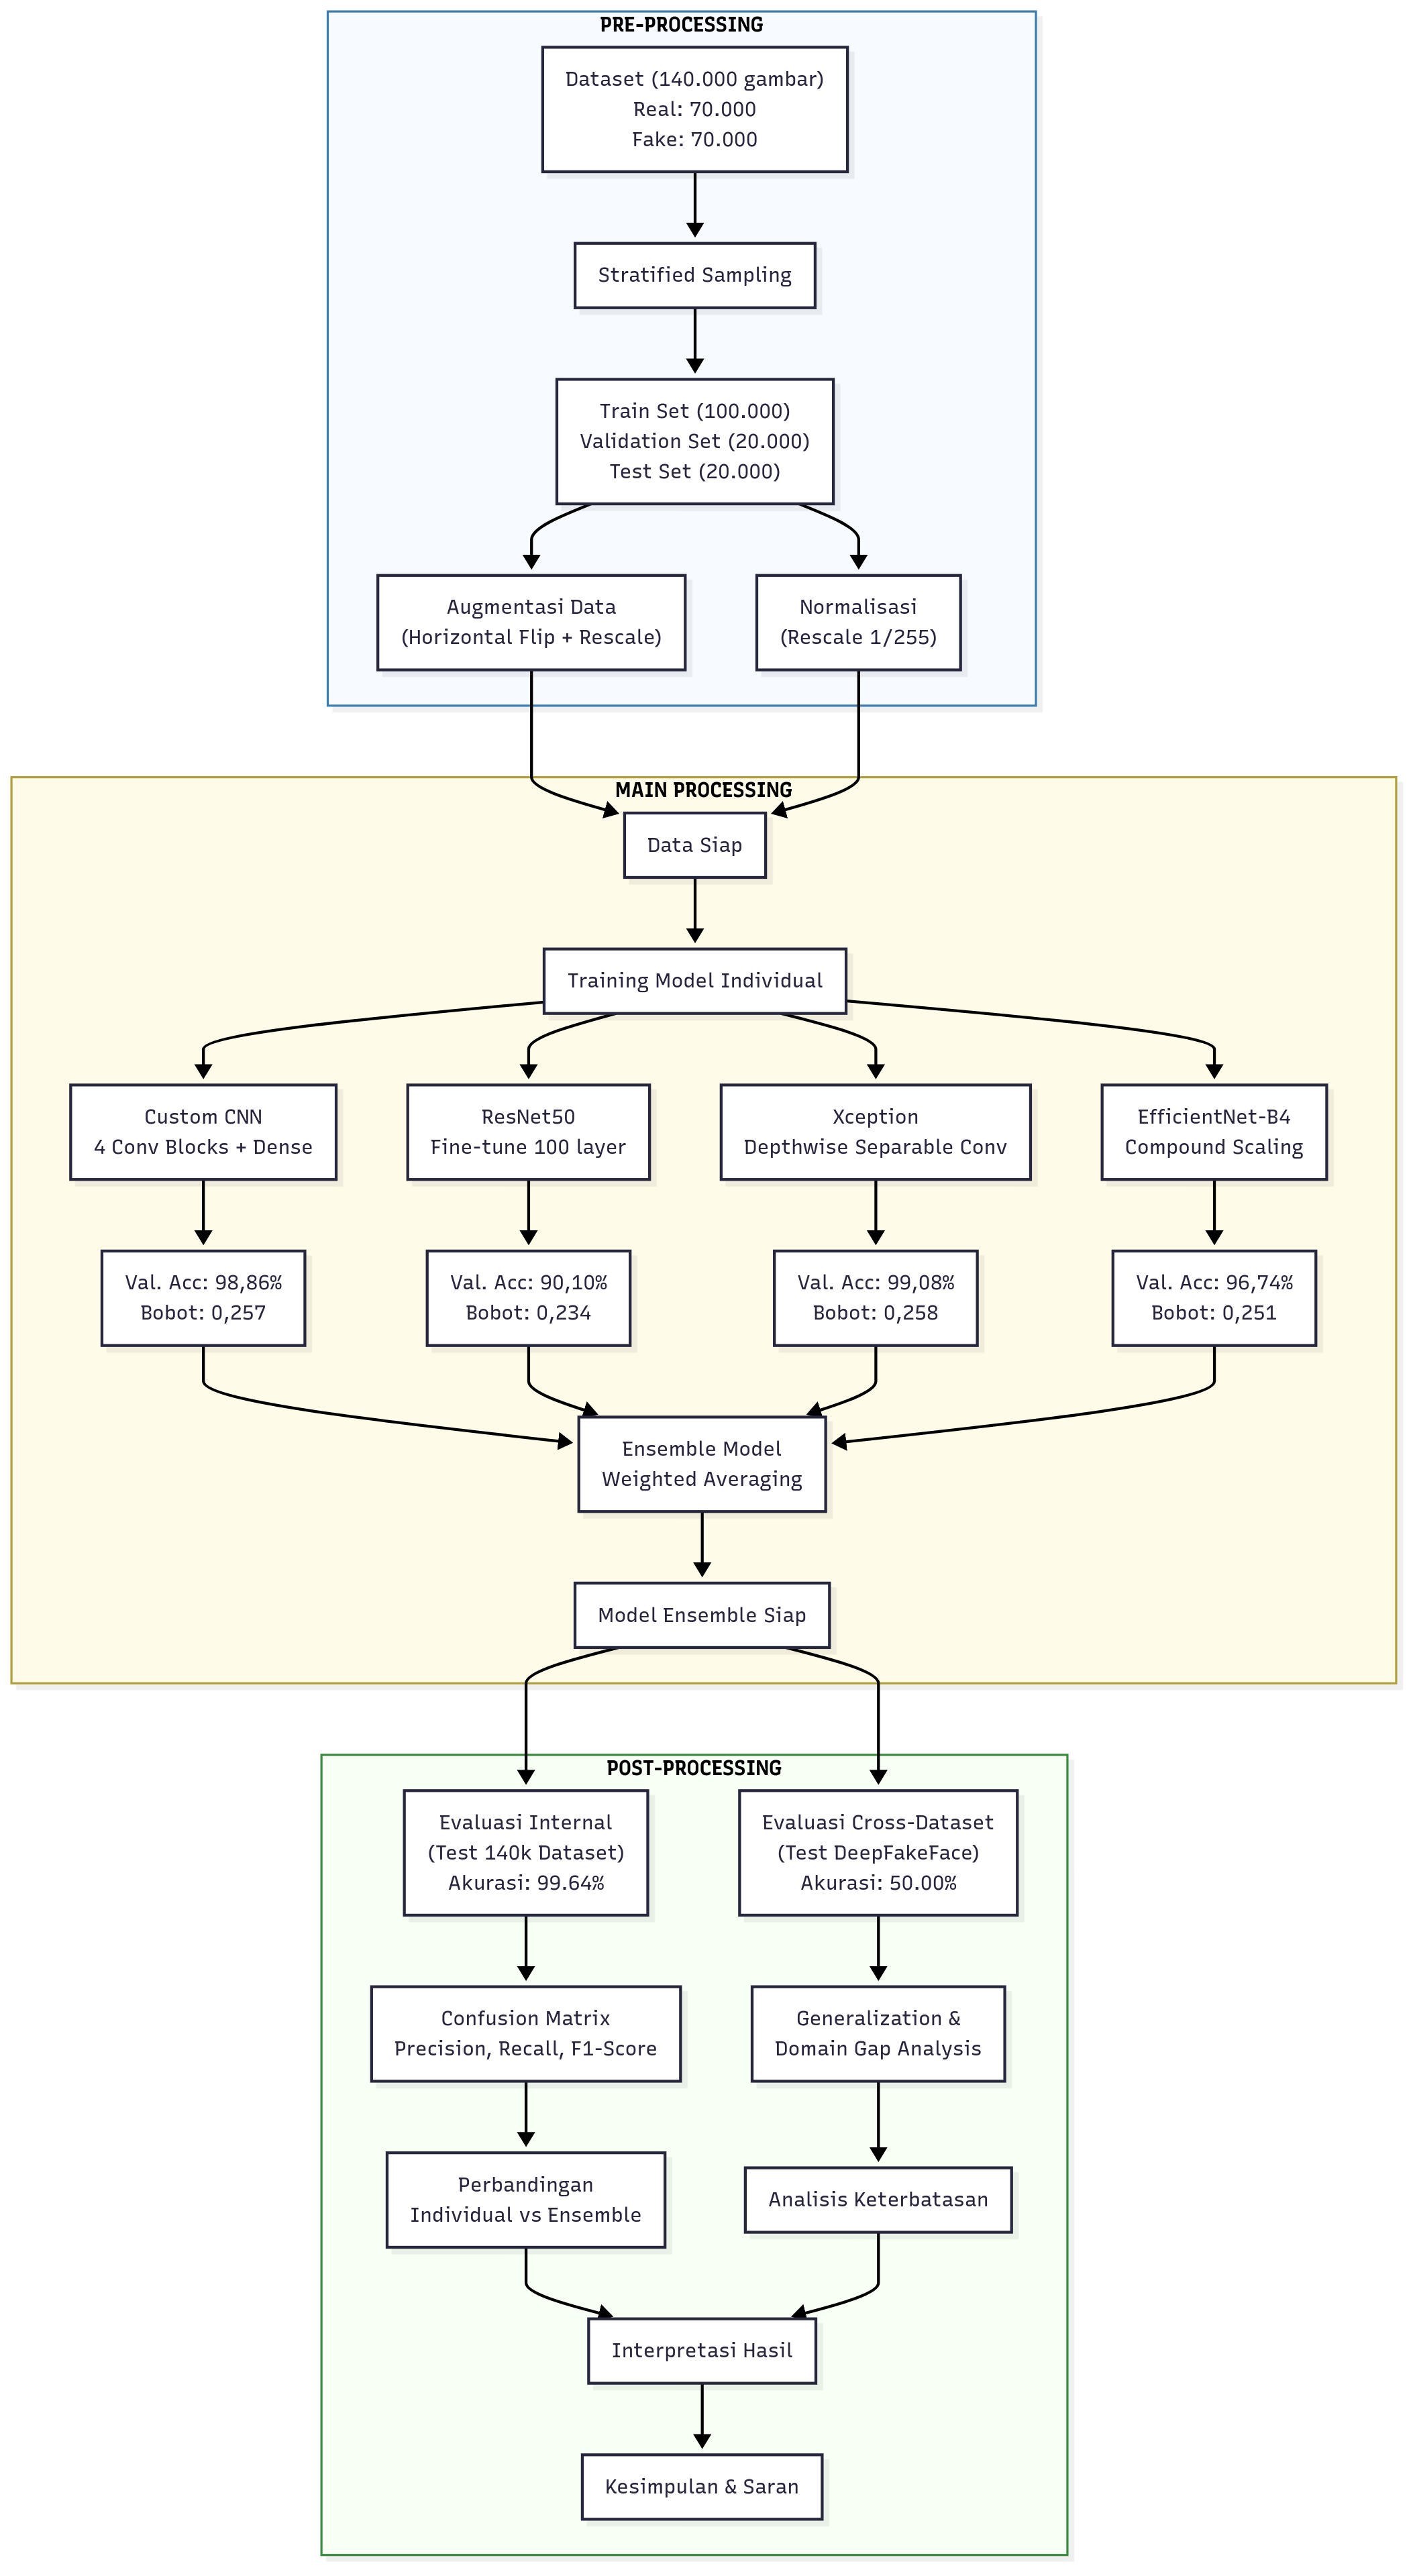
\includegraphics[width=0.85\textwidth]{assets/pics/pro-main-post.png}}
    \caption{Pipeline implementasi lengkap: pre-processing, main processing, dan post-processing}
    \label{fig:implementation_pipeline}
\end{figure}

Pipeline eksperimen ini terdiri dari tiga tahapan utama yang saling berkesinambungan:

\begin{enumerate}
    \item \textbf{Pre-processing (Tahap Biru)}: Meliputi akuisisi dataset "140k Real and Fake Faces" dengan komposisi seimbang 70.000 gambar asli dan 70.000 gambar palsu, stratified sampling untuk pembagian train/validation/test set, serta aplikasi augmentasi data minimal (horizontal flip) dan normalisasi (rescale 1/255) untuk mempertahankan artefak deteksi \textit{deepfake}.

    \item \textbf{Main Processing (Tahap Kuning)}: Merupakan inti eksperimen yang mencakup pelatihan empat model individual secara parallel (Custom CNN, ResNet50, Xception, EfficientNet-B4), penghitungan bobot ensemble berdasarkan validation accuracy menggunakan Persamaan~\ref{eq:performance_weight}, dan implementasi \textit{ensemble weighted averaging} sesuai Persamaan~\ref{eq:weighted_ensemble}.

    \item \textbf{Post-processing (Tahap Hijau)}: Evaluasi komprehensif melalui pengujian internal pada test set (akurasi 99,64\%), evaluasi cross-dataset menggunakan dataset eksternal DeepFakeFace (akurasi 50,0\%), analisis confusion matrix untuk memahami karakteristik kesalahan, perbandingan performa individual vs ensemble, dan interpretasi hasil untuk menjawab research questions.
\end{enumerate}

Setiap tahap dirancang dengan tujuan spesifik untuk menjawab research questions yang telah diformulasikan, dengan emphasis khusus pada komplementaritas model dalam tahap ensemble averaging. Hasil dari pipeline ini menunjukkan peningkatan performa yang konsisten dari model individual terbaik (Xception: 99,20\%) ke ensemble (99,64\%), dengan reduksi signifikan dalam false negatives dan false positives.

%-----------------------------------------------------------------------------%
\section{Hasil Pelatihan Model Individual}
%-----------------------------------------------------------------------------%
Tahap pertama dalam analisis adalah mengevaluasi performa dari masing-masing dari empat arsitektur yang dilatih secara individual. Bagian ini akan merinci hasil pelatihan, kurva pembelajaran, serta metrik evaluasi akhir pada \textit{dataset} pengujian untuk model \textit{Custom CNN}, \textit{ResNet50}, \textit{Xception}, dan \textit{EfficientNet-B4}. Hasil-hasil ini menjadi fondasi untuk pembobotan dan evaluasi sistem \textit{ensemble}.


\subsection{Performa Model CNN}

Model CNN yang dirancang khusus untuk deteksi \textit{deepfake} menunjukkan pembelajaran yang stabil tanpa menunjukkan hasil yang overfitting. Model mencapai konvergensi pada \textit{epoch} ke-12 dengan \textit{validation accuracy} tertinggi 98,86\%.

\begin{figure}[H]
    \centering
    \fbox{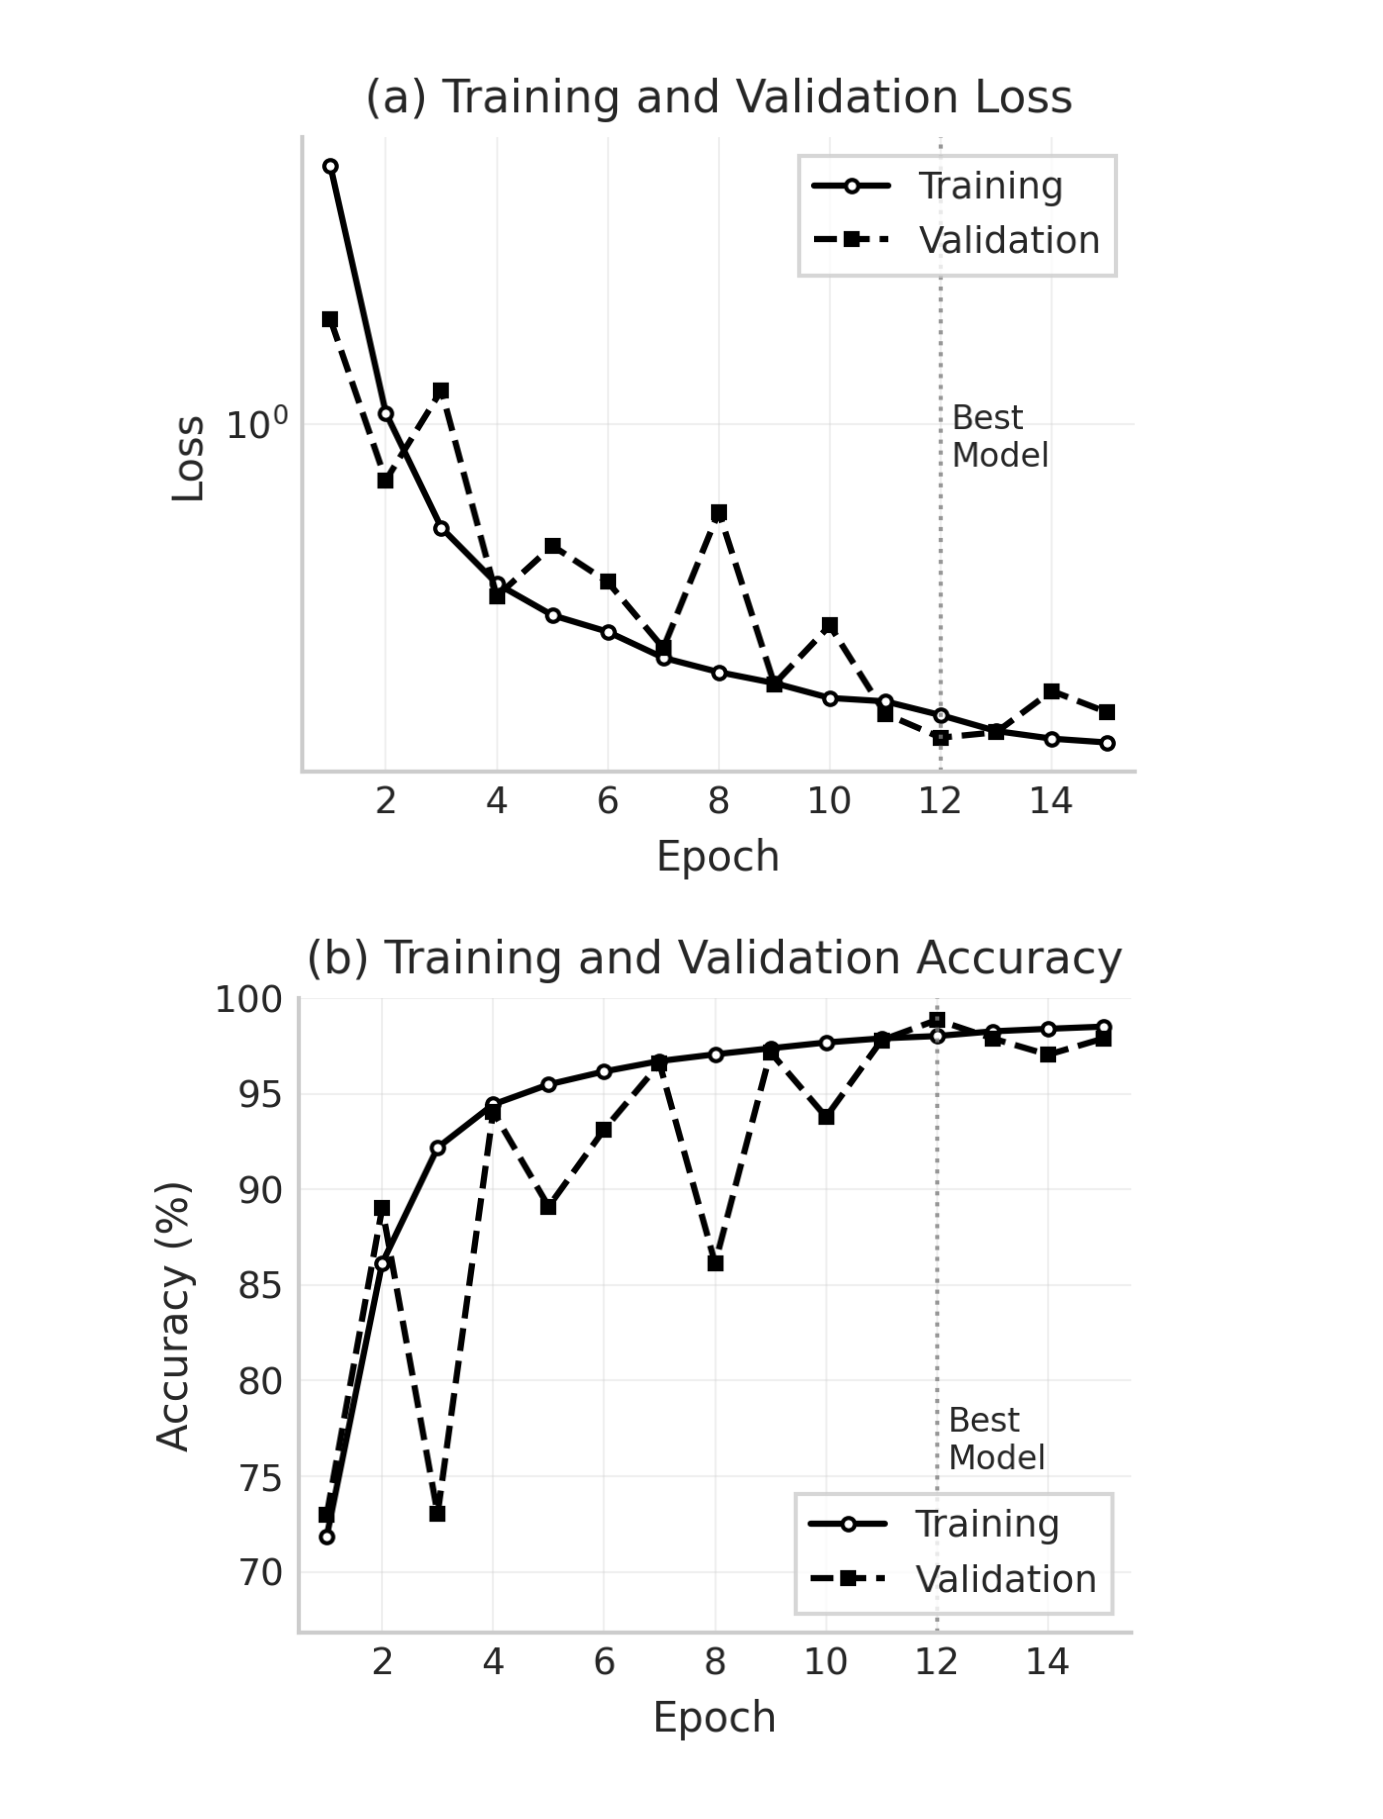
\includegraphics[width=0.6\textwidth]{assets/pics/cnn_training_curves (1).png}}
    \caption{Kurva pelatihan model \textit{CNN} menunjukkan \textit{loss} dan akurasi selama proses pembelajaran}
    \label{fig:cnn_training}
\end{figure}


Analisis kurva pelatihan pada Gambar~\ref{fig:cnn_training} menunjukkan bahwa model \textit{Custom CNN} mengalami pembelajaran yang konsisten dengan beberapa fluktuasi pada \textit{validation accuracy}, namun secara keseluruhan menunjukkan tren peningkatan yang baik.

\begin{table}[H]
\centering
\caption{Metrik evaluasi dari model CNN}
\label{tab:cnn_results}
\begin{tabular}{|l|c|}
\hline
\textbf{Metrik} & \textbf{Nilai} \\
\hline
\textit{Best Validation Accuracy} & 98,86\% \\
\textit{Test Accuracy} & 98,81\% \\
\textit{Test Precision} & 99,02\% \\
\textit{Test Recall} & 98,60\% \\
\textit{Test F1-Score} & 98,81\% \\
\hline
\end{tabular}
\end{table}

\subsection{Performa Model ResNet50}

Model \textit{ResNet50} dengan \textit{transfer learning} menunjukkan performa yang lebih rendah dari yang diharapkan. Meskipun menggunakan \textit{pre-trained weights} dari \textit{ImageNet}, model ini mengalami kesulitan dalam konvergensi dan menunjukkan tanda-tanda \textit{overfitting}.

\begin{figure}[H]
    \centering
    \fbox{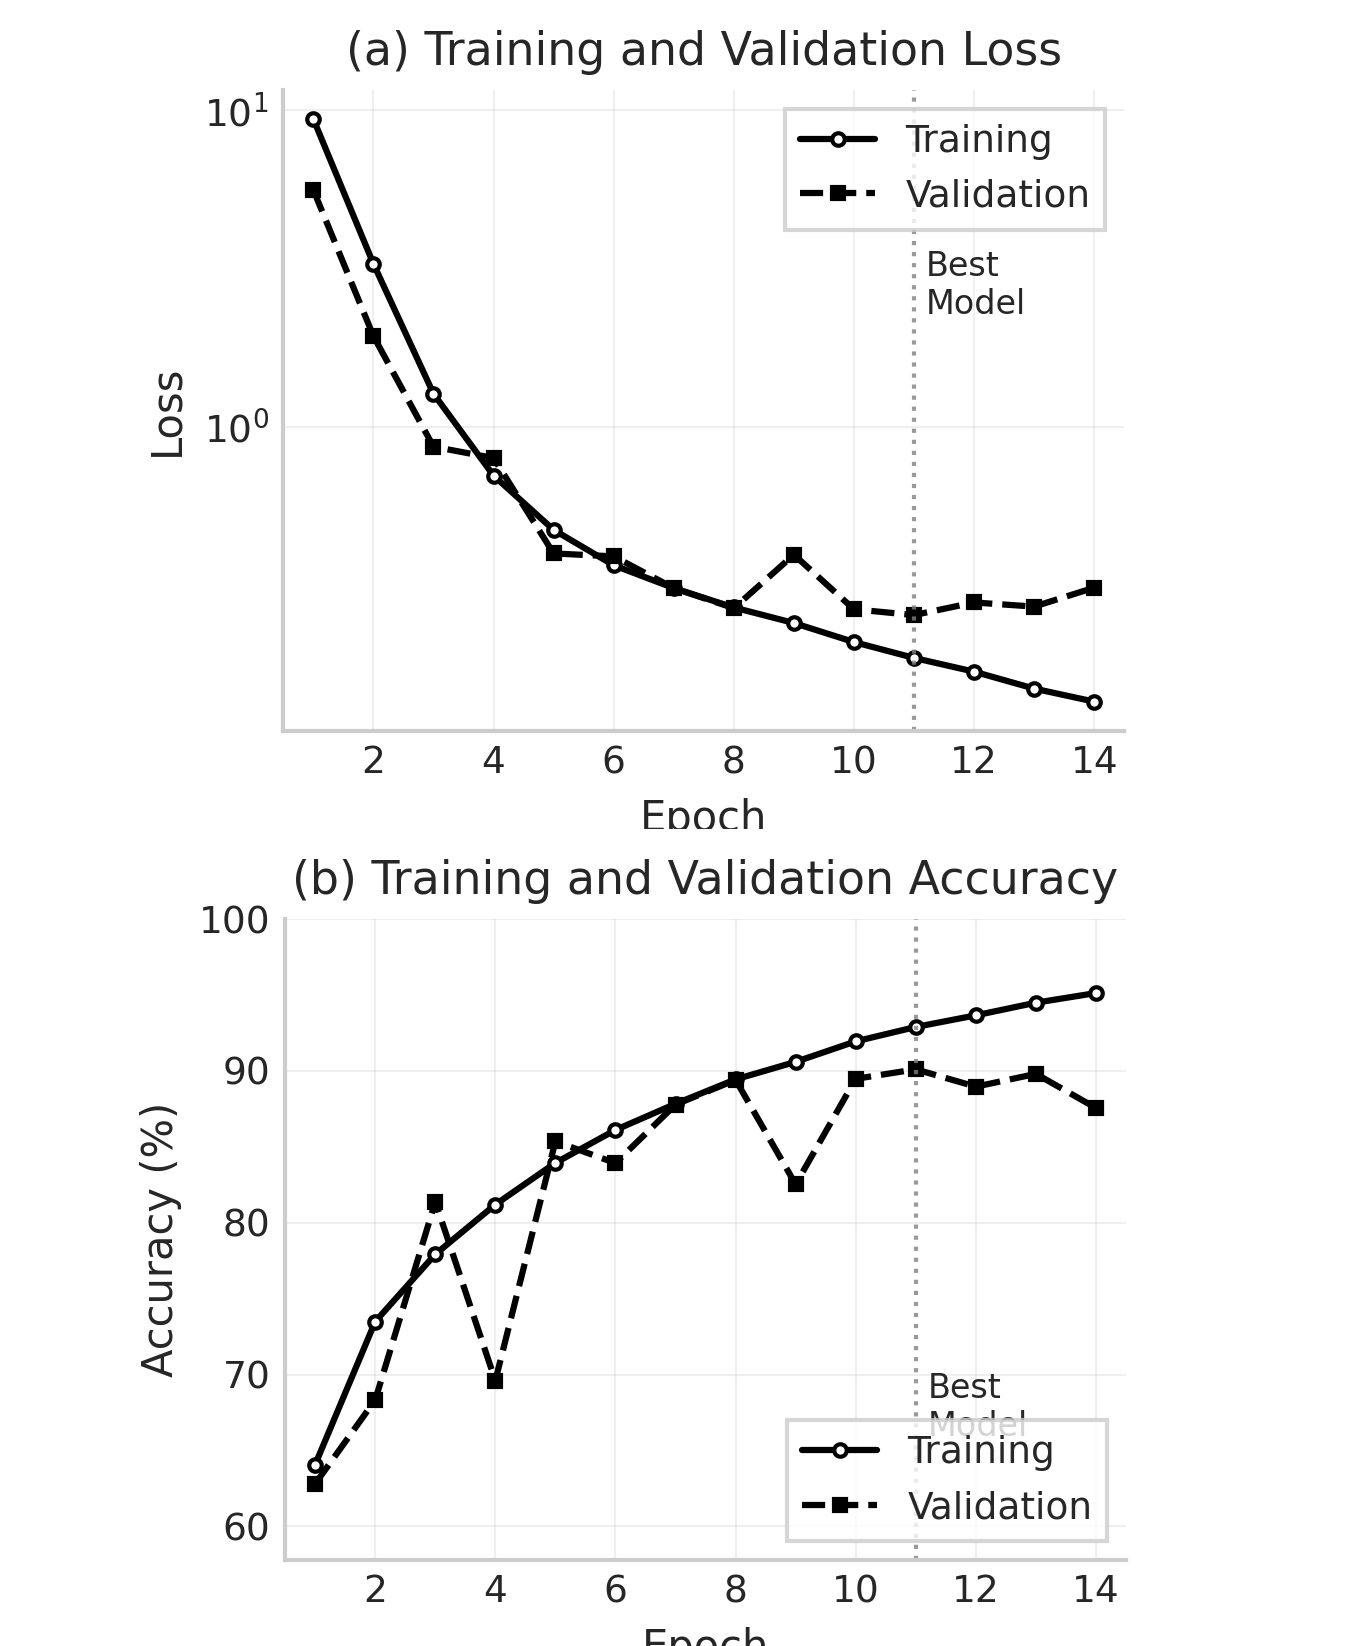
\includegraphics[width=0.6\textwidth]{assets/pics/resnet_training_curves (1).png}}
    \caption{Kurva pelatihan model \textit{ResNet50} dengan strategi \textit{transfer learning}}
    \label{fig:resnet_training}
\end{figure}

Kurva pelatihan pada Gambar~\ref{fig:resnet_training} menunjukkan fluktuasi yang signifikan pada \textit{validation accuracy} dan mencapai performa terbaik pada \textit{epoch} ke-11.

\begin{table}[H]
\centering
\caption{Metrik evaluasi dari model \textit{ResNet50}}
\label{tab:resnet_results}
\begin{tabular}{|l|c|}
\hline
\textbf{Metrik} & \textbf{Nilai} \\
\hline
\textit{Best Validation Accuracy} & 90,10\% \\
\textit{Test Accuracy} & 90,10\% \\
\textit{Test Precision} & 86,49\% \\
\textit{Test Recall} & 95,03\% \\
\textit{Test F1-Score} & 90,56\% \\
\hline
\end{tabular}
\end{table}

\subsection{Performa Model Xception}

Model \textit{Xception} dengan arsitektur \textit{depthwise separable convolution} menunjukkan performa terbaik di antara keempat model individual. Model mencapai konvergensi yang sangat baik dengan \textit{early stopping} pada \textit{epoch} ke-9 dan mempertahankan performa hingga \textit{epoch} ke-12.

\begin{figure}[H]
    \centering
    \fbox{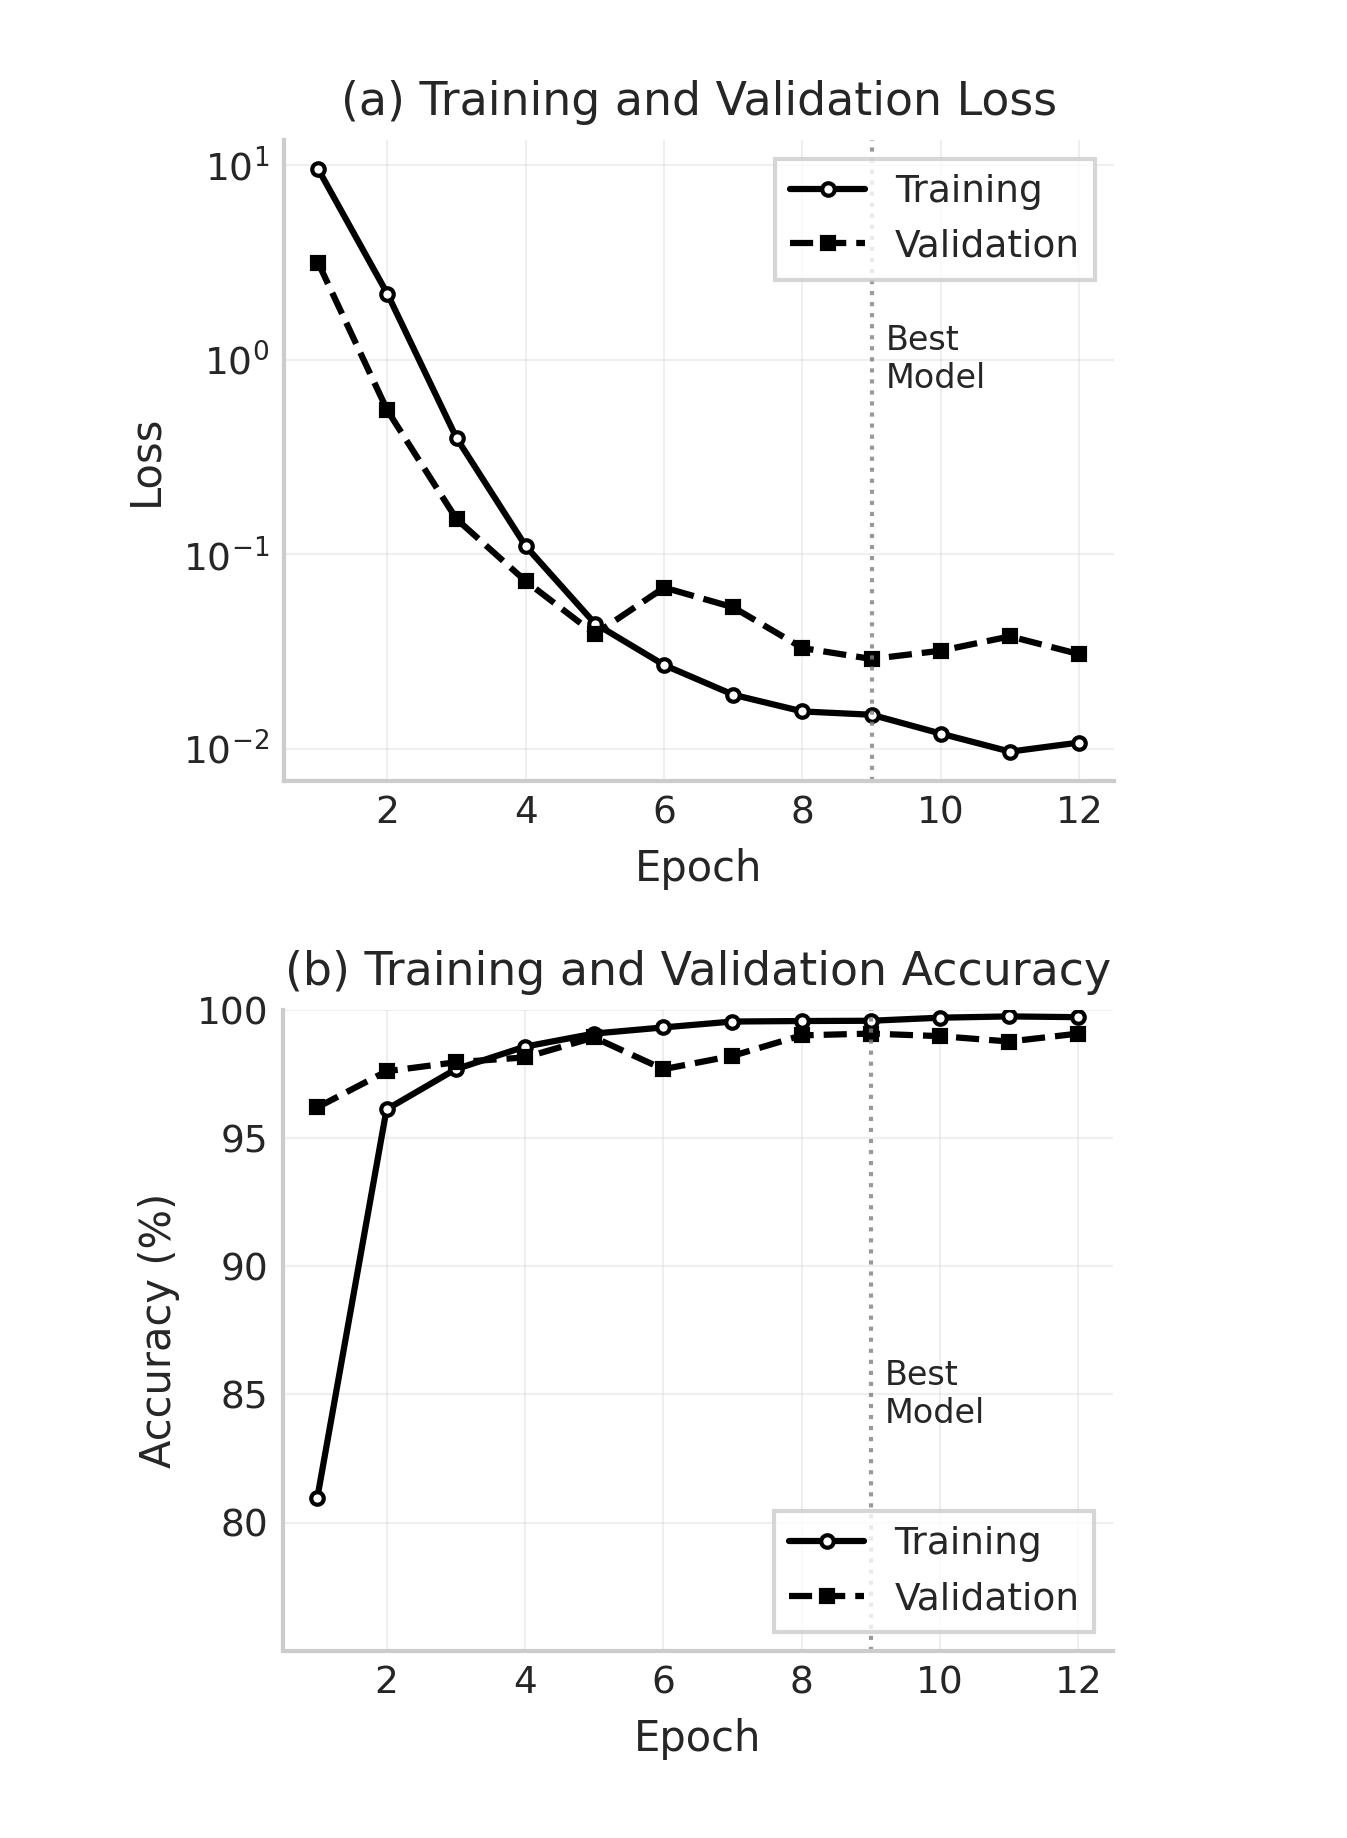
\includegraphics[width=0.6\textwidth]{assets/pics/xception_training_curves (1).png}}
    \caption{Kurva pelatihan model \textit{Xception} menunjukkan efisiensi pembelajaran yang superior}
    \label{fig:xception_training}
\end{figure}

Analisis pada Gambar~\ref{fig:xception_training} menunjukkan konvergensi yang sangat cepat dan stabil, dengan pencapaian akurasi tinggi pada \textit{epoch} awal dan mempertahankan stabilitas sepanjang proses pelatihan.

\begin{table}[H]
\centering
\caption{Metrik evaluasi dari model Xception}
\label{tab:xception_results}
\begin{tabular}{|l|c|}
\hline
\textbf{Metrik} & \textbf{Nilai} \\
\hline
\textit{Best Validation Accuracy} & 99,08\% \\
\textit{Test Accuracy} & 99,20\% \\
\textit{Test Precision} & 98,87\% \\
\textit{Test Recall} & 99,54\% \\
\textit{Test F1-Score} & 99,20\% \\
\hline
\end{tabular}
\end{table}

\subsection{Performa Model EfficientNet-B4}

Model \textit{EfficientNet-B4} dengan strategi \textit{compound scaling} menunjukkan pembelajaran yang stabil dan konsisten sepanjang 15 \textit{epoch}. Model mencapai performa optimal pada \textit{epoch} ke-14 dengan pembelajaran gradual yang tidak menunjukkan \textit{overfitting}.

\begin{figure}[H]
    \centering
    \fbox{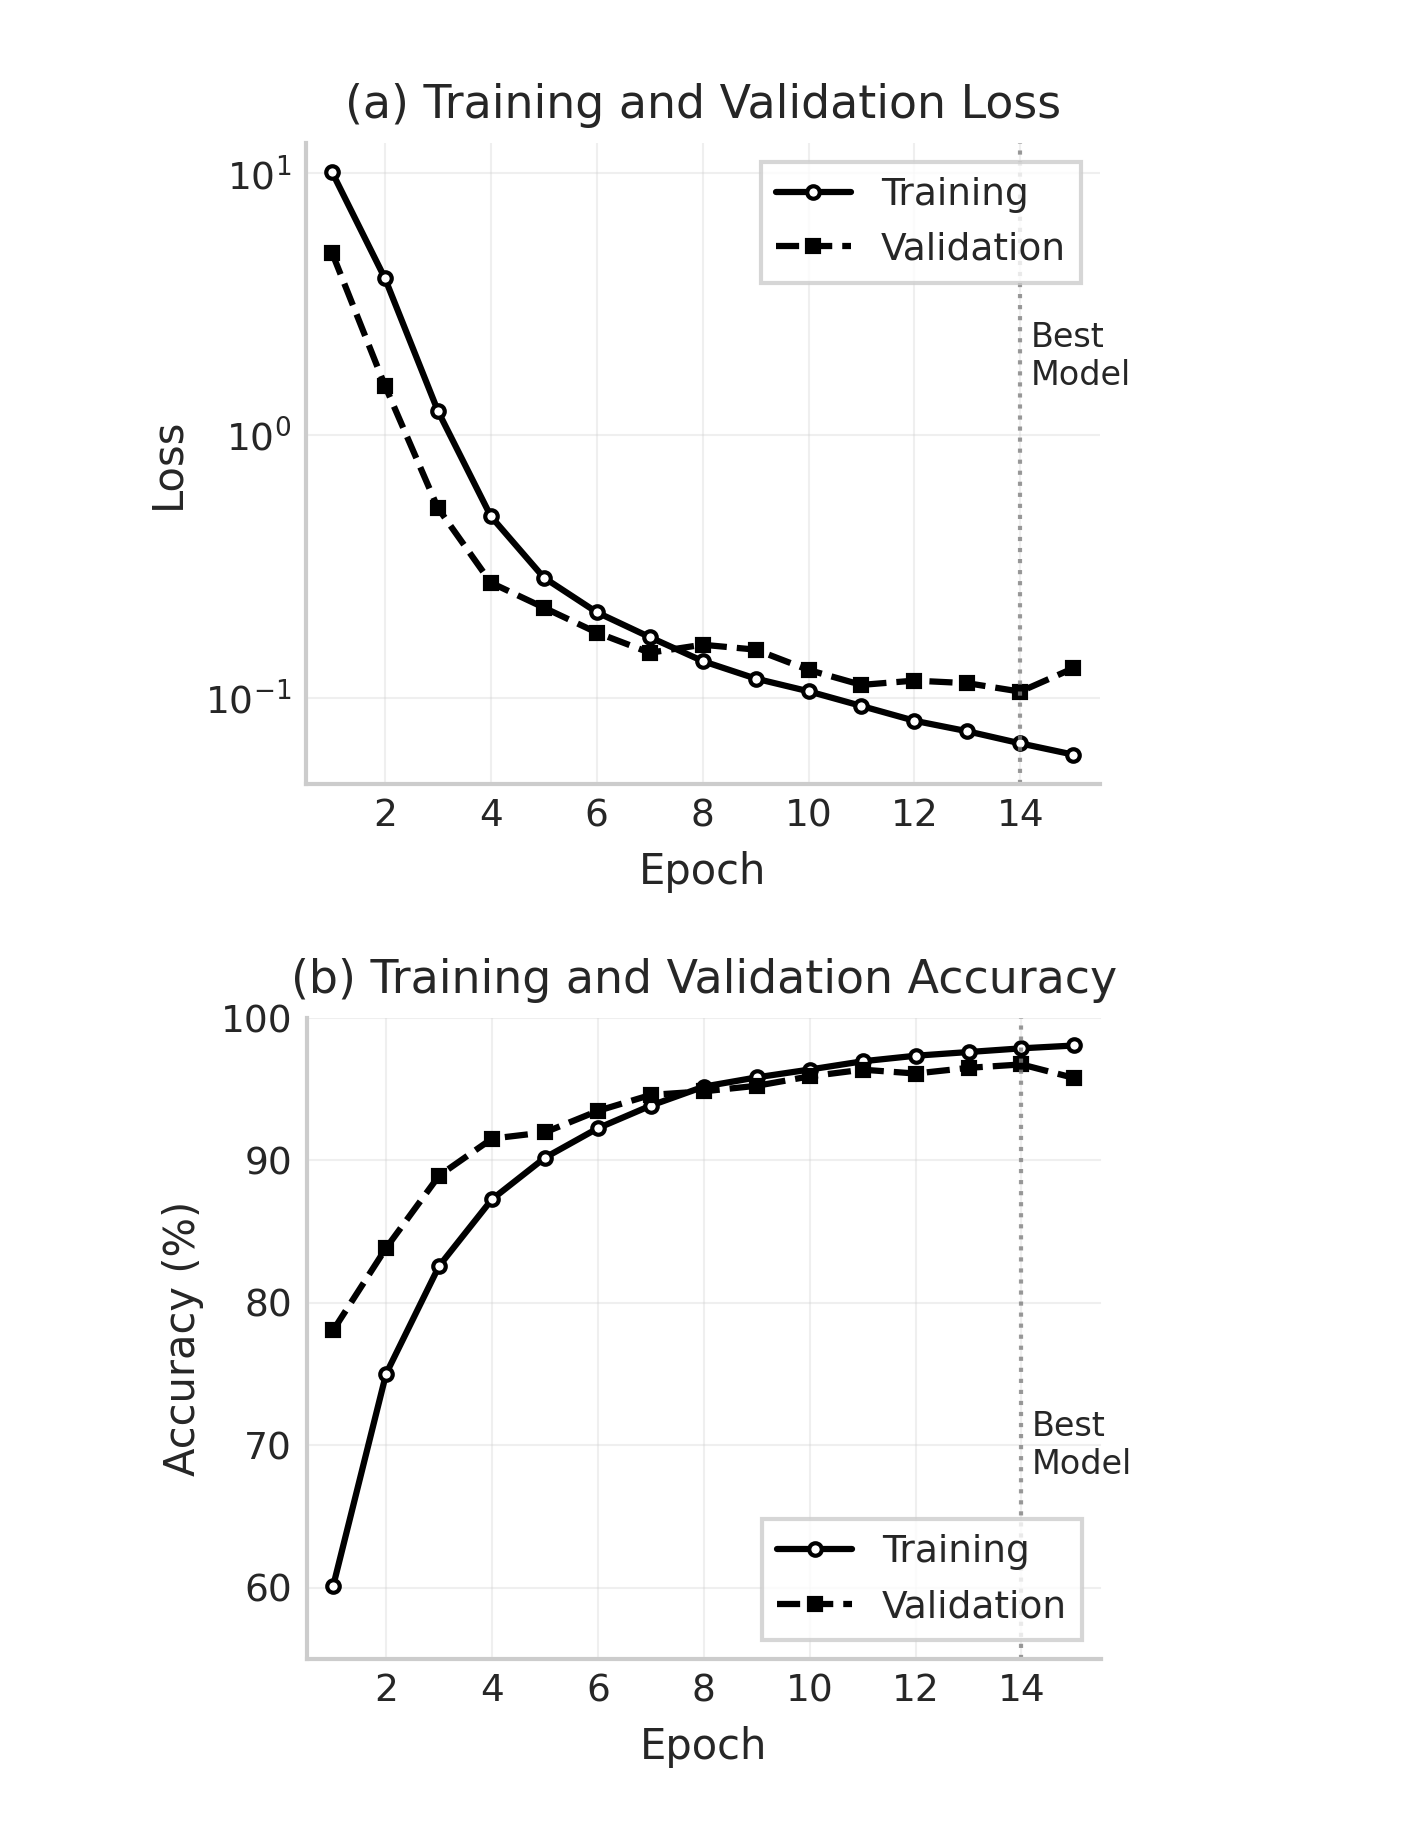
\includegraphics[width=0.6\textwidth]{assets/pics/efficientnet_training_curves (1).png}}
    \caption{Kurva pelatihan model \textit{EfficientNet-B4} dengan \textit{compound scaling}}
    \label{fig:efficientnet_training}
\end{figure}

Kurva pelatihan pada Gambar~\ref{fig:efficientnet_training} menunjukkan peningkatan yang steady dan konsisten tanpa fluktuasi yang signifikan, mengindikasikan pembelajaran yang stabil.

\begin{table}[H]
\centering
\caption{Metrik evaluasi dari model \textit{EfficientNet-B4}}
\label{tab:efficientnet_results}
\begin{tabular}{|l|c|}
\hline
\textbf{Metrik} & \textbf{Nilai} \\
\hline
\textit{Best Validation Accuracy} & 96,74\% \\
\textit{Test Accuracy} & 96,35\% \\
\textit{Test Precision} & 96,47\% \\
\textit{Test Recall} & 96,22\% \\
\textit{Test F1-Score} & 96,35\% \\
\hline
\end{tabular}
\end{table}

\subsection{Arsitektur Ensemble Akhir}

Bobot untuk setiap model dalam metode \textit{ensemble weighted averaging} dihitung berdasarkan performa akurasi terbaik dari masing-masing model pada saat proses validasi (\textit{validation accuracy}). Sesuai dengan formula yang dijelaskan dalam Persamaan~\ref{eq:weight_calculation} pada Bab 2, bobot dinormalisasi sehingga totalnya menjadi 1. Proses perhitungan bobot ini dirangkum pada Tabel \ref{tab:ensemble_weights}.

\begin{table}[H]
    \centering
    \caption{Perhitungan bobot ensemble berdasarkan akurasi validasi}
    \label{tab:ensemble_weights}
    \begin{tabular}{|l|c|c|}
        \hline
        \textbf{Arsitektur Model} & \textbf{Akurasi Validasi Terbaik (\%)} & \textbf{Bobot Ensemble Final ($w_i$)} \\
        \hline
        Custom CNN & 98{,}86 & 0{,}257 \\
        ResNet50 & 90{,}10 & 0{,}234 \\
        Xception & 99{,}08 & 0{,}258 \\
        EfficientNet-B4 & 96{,}74 & 0{,}251 \\
        \hline
        \textbf{Total} & \textbf{384{,}78} & \textbf{1{,}000} \\
        \hline
    \end{tabular}
\end{table}

Berdasarkan bobot yang telah dihitung menggunakan metodologi yang dijelaskan pada Bab 3, formula final untuk implementasi \textit{ensemble weighted averaging} pada penelitian ini mengikuti Persamaan~\ref{eq:weighted_ensemble} sebagai berikut:

\begin{equation}
\hat{y}_{\text{ensemble}}(x) = 0{,}257 \cdot \hat{y}_{\text{CNN}}(x) + 0{,}234 \cdot \hat{y}_{\text{ResNet}}(x) + 0{,}258 \cdot \hat{y}_{\text{Xception}}(x) + 0{,}251 \cdot \hat{y}_{\text{EfficientNet}}(x)
\label{eq:final_ensemble}
\end{equation}

Nilai bobot tertinggi diberikan kepada model Xception yang memiliki akurasi validasi tertinggi, sementara bobot terendah diberikan kepada ResNet50 yang menunjukkan akurasi validasi paling rendah.


%-----------------------------------------------------------------------------%
\section{Evaluasi Komprehensif dan Perbandingan}
%-----------------------------------------------------------------------------%

Puncak dari eksperimen ini adalah evaluasi komprehensif untuk mengukur efektivitas sistem \textit{ensemble} yang telah dibangun. Bagian ini menyajikan perbandingan langsung antara performa model \textit{ensemble} dengan keempat model individual pada metrik-metrik kunci. Analisis \textit{confusion matrix} juga disertakan untuk memberikan pemahaman mendalam mengenai karakteristik dan distribusi \textit{error} dari setiap model.

\subsection{Hasil Evaluasi Ensemble}

Sistem \textit{ensemble weighted averaging} menunjukkan peningkatan performa dibandingkan dengan model individual terbaik:

\begin{table}[h]
\centering
\caption{Hasil evaluasi model \textit{ensemble} dan model individual}
\label{tab:comprehensive_results}
\begin{tabular}{|l|c|c|c|c|}
\hline
\textbf{Model} & \textbf{Accuracy} & \textbf{Precision} & \textbf{Recall} & \textbf{F1-Score}  \\
\hline
\textit{CNN} & 98,81\% & 99,02\% & 98,60\% & 98,81\% \\
\textit{ResNet50} & 90,10\% & 86,49\% & 95,03\% & 90,56\%  \\
\textit{Xception} & 99,20\% & 98,87\% & 99,54\% & 99,20\%  \\
\textit{EfficientNet-B4} & 96,35\% & 96,47\% & 96,22\% & 96,35\%  \\
\hline
\textbf{\textit{Ensemble}} & \textbf{99,64\%} & \textbf{99,39\%} & \textbf{99,90\%} & \textbf{99,65\%}  \\
\hline
\end{tabular}
\end{table}

Dari Tabel~\ref{tab:comprehensive_results}, dapat diamati bahwa model ensemble secara konsisten mengungguli semua model individual dalam semua metrik evaluasi yang telah didefinisikan dalam Persamaan~\ref{eq:accuracy}, \ref{eq:precision}, \ref{eq:recall}, dan \ref{eq:f1score} pada Bab 2.

\subsection{Analisis Keseimbangan Metrik Kinerja}

Meskipun metrik Akurasi (Persamaan~\ref{eq:accuracy}) memberikan gambaran umum performa model, analisis yang lebih mendalam terhadap Presisi (Persamaan~\ref{eq:precision}) dan Perolehan/\textit{Recall} (Persamaan~\ref{eq:recall}) dapat menyajikan evaluasi yang lebih komprehensif, terutama pada kasus penggunaan dengan konsekuensi kesalahan yang signifikan seperti deteksi \textit{deepfake}. Kedua metrik ini menguraikan \textit{trade-off} yang melekat pada sistem klasifikasi:

\begin{itemize}
    \item \textbf{Presisi} mengukur proporsi prediksi positif yang benar dari total prediksi positif yang dibuat. Dalam konteks ini, Presisi yang tinggi (99,39\% pada model \textit{ensemble}) mengindikasikan bahwa ketika model mengklasifikasikan sebuah gambar sebagai \textit{deepfake}, klaim tersebut memiliki tingkat kebenaran yang tinggi. Implikasi praktisnya adalah rendahnya angka \textit{False Positive}, sehingga dapat meminimalkan risiko pemblokiran terhadap konten yang sah.

    \item \textbf{Perolehan (\textit{Recall})} mengukur kapabilitas model dalam mengidentifikasi seluruh sampel positif aktual dari dataset. Perolehan yang tinggi (99,90\% pada model \textit{ensemble}) menunjukkan bahwa model mampu menangkap mayoritas konten \textit{deepfake} yang ada. Implikasi praktisnya adalah rendahnya angka \textit{False Negative}, yang merupakan aspek krusial untuk memitigasi risiko penyebaran konten manipulatif.
\end{itemize}

Berdasarkan data pada Tabel 4.5, model individual dengan kinerja terbaik, Xception, menunjukkan \textit{trade-off} di mana nilai Perolehan (99,54\%) lebih tinggi daripada Presisi (98,87\%). Hal ini mengindikasikan sensitivitas deteksi yang tinggi, namun dengan kerentanan yang sedikit lebih besar terhadap klasifikasi positif yang keliru.

Model \textit{ensemble} yang diusulkan tidak hanya meningkatkan kedua metrik tersebut secara absolut, tetapi juga mencapai keseimbangan yang lebih optimal. Dengan nilai Presisi 99,39\% dan Perolehan 99,90\%, model \textit{ensemble} menunjukkan tingkat keandalan dan efektivitas yang tinggi, yang tercermin dari rendahnya angka kesalahan klasifikasi pada kedua kelas. Nilai F1-Score tertinggi yang dicapainya (99,65\%) yang dihitung menggunakan Persamaan~\ref{eq:f1score} secara matematis mengonfirmasi keunggulan model \textit{ensemble} dalam menyeimbangkan kedua aspek krusial ini.

%-----------------------------------------------------------------------------%
\section{Analisis Confusion Matrix dan Karakteristik Model}
%-----------------------------------------------------------------------------%

Bagian ini menyajikan analisis mendalam terhadap \textit{confusion matrix} masing-masing model untuk memahami karakteristik kesalahan (error profile) yang berbeda-beda. Analisis individual ini memberikan wawasan penting mengenai komplementaritas antar model yang menjadi landasan keberhasilan pendekatan \textit{ensemble}.

\subsection{Analisis Custom CNN}

Model Custom CNN menunjukkan performa yang seimbang dengan karakteristik kesalahan yang dapat diprediksi. Gambar~\ref{fig:conf_matrix_cnn} menampilkan distribusi prediksi pada dataset pengujian.

\begin{figure}[H]
    \centering
    \fbox{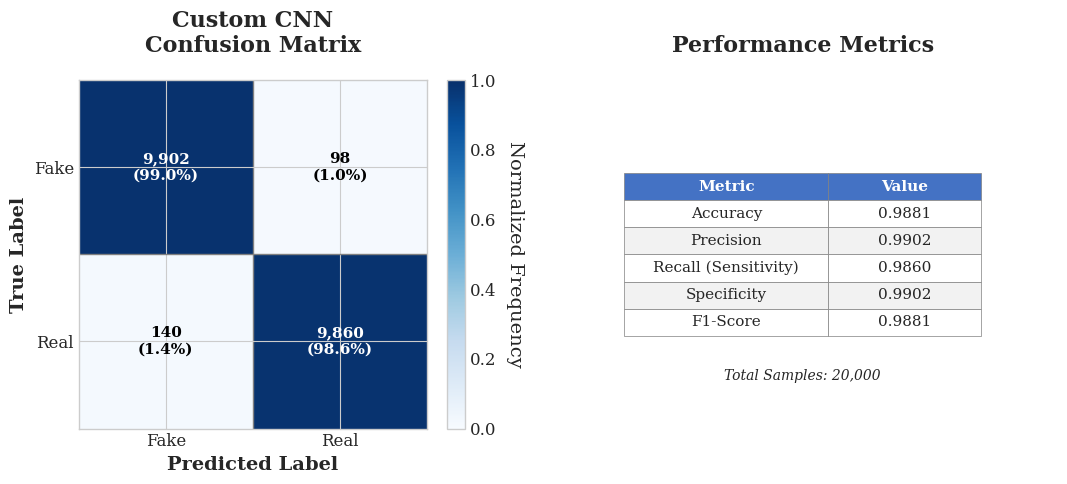
\includegraphics[width=0.85\textwidth]{assets/pics/cnn_confusion_matrix.png}}
    \caption{Confusion matrix dan metrik performa model Custom CNN menunjukkan keseimbangan yang baik antara precision dan recall dengan akurasi 98,81\%}
    \label{fig:conf_matrix_cnn}
\end{figure}

Berdasarkan analisis confusion matrix, model Custom CNN memiliki karakteristik sebagai berikut:
\begin{itemize}
    \item \textbf{False Negative}: 140 kasus (1,4\%) - Model cenderung lebih konservatif dalam mengklasifikasi deepfake
    \item \textbf{False Positive}: 98 kasus (1,0\%) - Tingkat kesalahan yang rendah dalam mengklasifikasi citra asli sebagai palsu
    \item \textbf{Karakteristik}: Menunjukkan keseimbangan yang baik antara sensitivity dan specificity
\end{itemize}

\subsection{Analisis ResNet50}

Model ResNet50 menunjukkan performa terlemah di antara semua model individual dengan pola kesalahan yang signifikan. Gambar~\ref{fig:conf_matrix_resnet50} mengungkapkan tantangan yang dihadapi model ini.

\begin{figure}[H]
    \centering
    \fbox{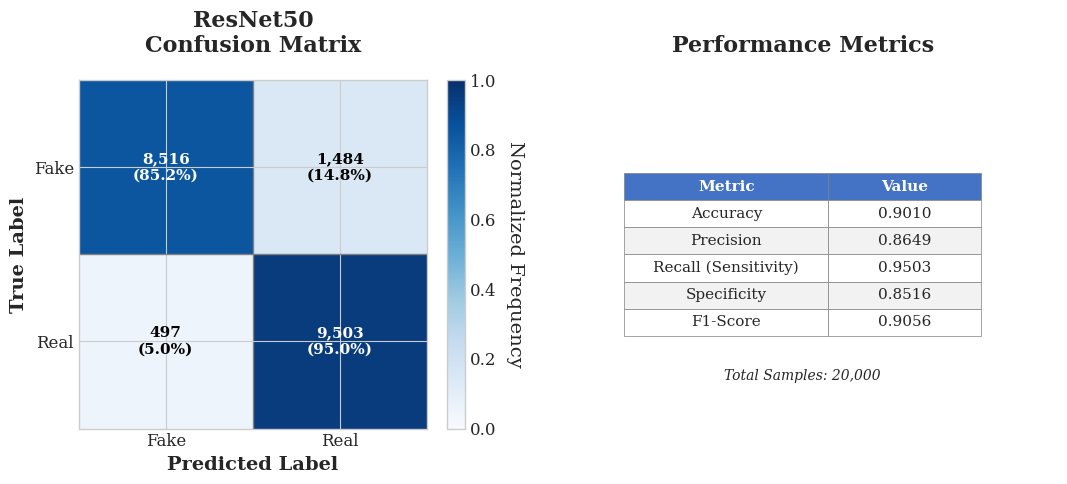
\includegraphics[width=0.85\textwidth]{assets/pics/resnet_confusion_matrix.png}}
    \caption{Confusion matrix dan metrik performa model ResNet50 menunjukkan tingkat false positive yang tinggi dengan akurasi 90,10\%, mengindikasikan overfitting pada domain transfer learning}
    \label{fig:conf_matrix_resnet50}
\end{figure}

ResNet50 memperlihatkan karakteristik kesalahan yang ekstrem:
\begin{itemize}
    \item \textbf{False Positive}: 1.484 kasus (14,8\%) - Sangat agresif dalam mengklasifikasi citra asli sebagai deepfake
    \item \textbf{False Negative}: 497 kasus (5,0\%) - Juga mengalami kesulitan dalam mendeteksi deepfake yang sebenarnya
    \item \textbf{Karakteristik}: Menunjukkan tanda-tanda overfitting dan adaptasi yang kurang optimal pada domain deteksi deepfake
\end{itemize}

\subsection{Analisis Xception}

Model Xception menunjukkan performa terbaik di antara model individual dengan sensitivitas deteksi yang sangat tinggi. Gambar~\ref{fig:conf_matrix_xception} menampilkan keunggulan model ini.

\begin{figure}[H]
    \centering
    \fbox{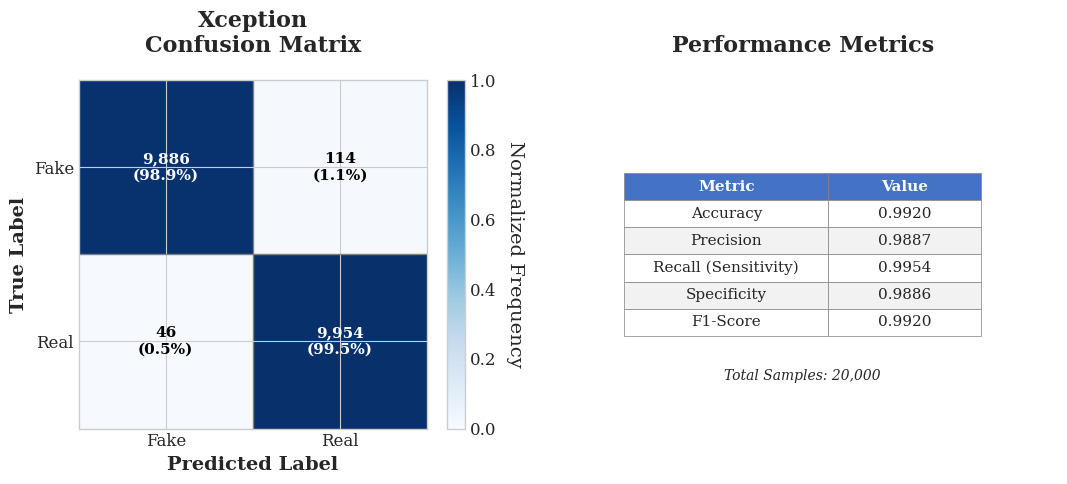
\includegraphics[width=0.85\textwidth]{assets/pics/xception_confusion_matrix.png}}
    \caption{Confusion matrix dan metrik performa model Xception menunjukkan tingkat recall tertinggi (99,54\%) dengan akurasi 99,20\%, namun dengan trade-off pada precision}
    \label{fig:conf_matrix_xception}
\end{figure}

Xception memperlihatkan karakteristik unggul dengan beberapa nuansa:
\begin{itemize}
    \item \textbf{False Negative}: 46 kasus (0,5\%) - Sangat efektif dalam mendeteksi deepfake
    \item \textbf{False Positive}: 114 kasus (1,1\%) - Sensitivitas tinggi menyebabkan kecenderungan over-detection
    \item \textbf{Karakteristik}: Model dengan bias detection yang tinggi, sangat baik untuk aplikasi yang memprioritaskan deteksi komprehensif
\end{itemize}

\subsection{Analisis EfficientNet-B4}

Model EfficientNet-B4 menunjukkan distribusi kesalahan yang relatif seimbang dengan performa yang stabil. Gambar~\ref{fig:conf_matrix_efficientnet} menggambarkan karakteristik model ini.

\begin{figure}[H]
    \centering
    \fbox{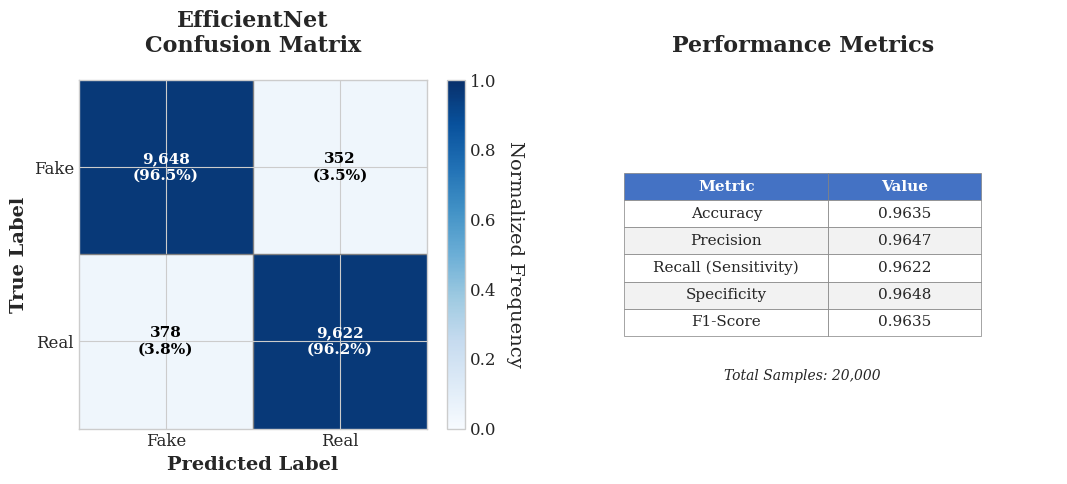
\includegraphics[width=0.85\textwidth]{assets/pics/efficientNet_confusion_matrix.png}}
    \caption{Confusion matrix dan metrik performa model EfficientNet-B4 menunjukkan keseimbangan antara false positive dan false negative dengan akurasi 96,35\%}
    \label{fig:conf_matrix_efficientnet}
\end{figure}

EfficientNet-B4 memperlihatkan profil kesalahan yang seimbang:
\begin{itemize}
    \item \textbf{False Negative}: 378 kasus (3,8\%) - Tingkat kesalahan moderat dalam mendeteksi deepfake
    \item \textbf{False Positive}: 352 kasus (3,5\%) - Tingkat kesalahan yang sebanding dalam mengklasifikasi citra asli
    \item \textbf{Karakteristik}: Model dengan pendekatan konservatif dan keseimbangan error yang dapat diprediksi
\end{itemize}

\subsection{Analisis Weighted Ensemble}

Model ensemble menunjukkan peningkatan performa yang signifikan dengan menggabungkan kekuatan semua model individual. Gambar~\ref{fig:conf_matrix_ensemble} mendemonstrasikan keunggulan pendekatan ensemble.

\begin{figure}[H]
    \centering
    \fbox{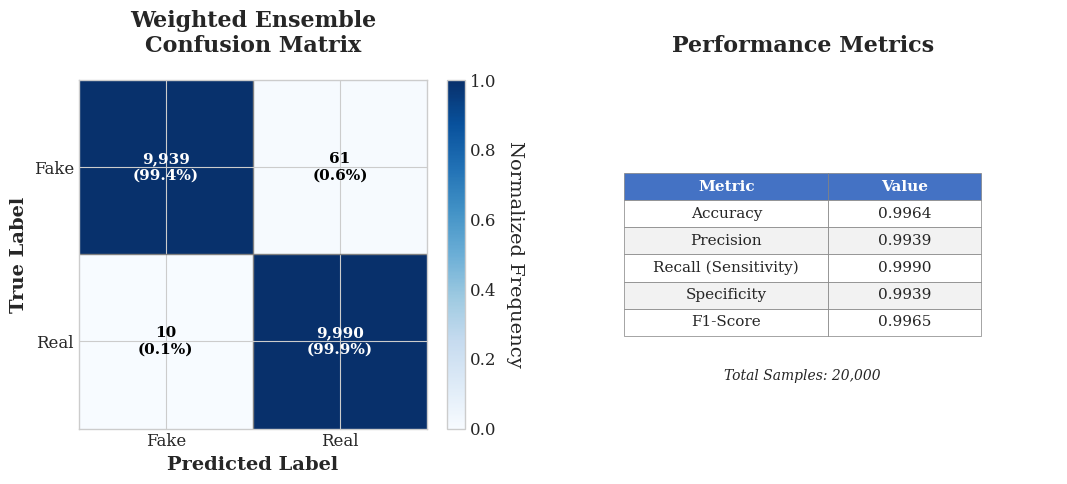
\includegraphics[width=0.85\textwidth]{assets/pics/weighted-ensemble_confusion_matrix.png}}
    \caption{Confusion matrix dan metrik performa model Weighted Ensemble menunjukkan performa superior dengan akurasi 99,64\%, recall 99,90\%, dan reduksi signifikan pada kedua jenis kesalahan}
    \label{fig:conf_matrix_ensemble}
\end{figure}

Weighted Ensemble menunjukkan optimalisasi yang luar biasa:
\begin{itemize}
    \item \textbf{False Negative}: 10 kasus (0,1\%) - Reduksi 78\% dari model individual terbaik (Xception)
    \item \textbf{False Positive}: 61 kasus (0,6\%) - Reduksi 46,5\% dari model individual terbaik (Xception)
    \item \textbf{Karakteristik}: Mencapai keseimbangan optimal antara sensitivity dan specificity
\end{itemize}

\subsection{Komplementaritas dan Perbandingan Keseluruhan}

Analisis individual menunjukkan pola komplementaritas yang jelas antar model, sebagaimana dirangkum dalam Tabel~\ref{tab:error_analysis_summary}.

\begin{table}[H]
\centering
\caption{Ringkasan analisis kesalahan dan karakteristik model}
\label{tab:error_analysis_summary}
\begin{tabular}{|l|c|c|c|l|}
\hline
\textbf{Model} & \textbf{FN} & \textbf{FP} & \textbf{Total Error} & \textbf{Karakteristik Utama} \\
\hline
Custom CNN & 140 & 98 & 238 & Konservatif, seimbang \\
ResNet50 & 497 & 1.484 & 1.981 & Agresif, tidak stabil \\
Xception & 46 & 114 & 160 & Sensitif, bias detection \\
EfficientNet-B4 & 378 & 352 & 730 & Moderat, prediktabel \\
\hline
\textbf{Ensemble} & \textbf{10} & \textbf{61} & \textbf{71} & \textbf{Optimal, robust} \\
\hline
\end{tabular}
\end{table}

Temuan ini secara empiris memvalidasi hipotesis komplementaritas model:
\begin{enumerate}
    \item \textbf{Diversitas Error Pattern}: Setiap model memiliki kecenderungan kesalahan yang berbeda, memungkinkan koreksi mutual
    \item \textbf{Kompensasi Kelemahan}: Kecenderungan over-detection Xception dikompensasi oleh konservatisme CNN dan EfficientNet
    \item \textbf{Stabilitas Ensemble}: Weighted averaging berhasil mengoptimalkan kontribusi setiap model sesuai dengan kemampuannya
    \item \textbf{Reduksi Risiko}: Ensemble secara signifikan mengurangi risiko false negative (critical miss) dan false positive (false alarm)
\end{enumerate}


%-----------------------------------------------------------------------------%
\section{Analisis Karakteristik dan Komplementaritas Model}
%-----------------------------------------------------------------------------%
Di balik angka-angka performa, terdapat karakteristik unik dari setiap model yang berkontribusi pada keberhasilan \textit{ensemble}. Bagian ini menggali lebih dalam untuk menganalisis temuan-temuan yang mengejutkan dari performa model individual dan, yang terpenting, menguraikan bagaimana perbedaan (komplementaritas) dalam kekuatan dan kelemahan setiap model memungkinkan \textit{ensemble} untuk mencapai tingkat akurasi yang lebih tinggi.

\subsection{Analisis Performa Model Individual}

Hasil eksperimen menunjukkan beberapa temuan yang menarik dan berbeda dari ekspektasi awal:

\begin{enumerate}
    \item \textbf{\textit{CNN} :} Model \textit{CNN} yang  mencapai akurasi 98,81\%, menunjukkan performa tinggi yang mendekati \textit{Xception}. Hal ini menunjukkan bahwa arsitektur CNN telah dirancang dengan baik dan mampu menyaingi model \textit{pretrained}.
    
    \item \textbf{\textit{ResNet50}:} \textit{ResNet50} menunjukkan performa terendah dengan akurasi hanya 90,10\%. Hal ini kemungkinan disebabkan oleh:
    \begin{itemize}
        \item Kompleksitas arsitektur yang tidak sesuai dengan karakteristik \textit{dataset}
        \item Strategi \textit{fine-tuning} yang kurang optimal
        \item \textit{Overfitting} yang terindikasi dari \textit{generalization gap} 2,79\%
    \end{itemize}
    
    \item \textbf{\textit{Xception}:} \textit{Xception} mencapai performa tertinggi (99,20\%) dengan efisiensi training yang sangat baik, memerlukan waktu pelatihan 71,5 menit untuk 12 \textit{epoch}.).
\end{enumerate}

\subsection{Efektivitas Weighted Averaging}

Peningkatan dari model individual terbaik (\textit{Xception}: 99,20\%) ke \textit{ensemble} (99,64\%) sebesar 0,44\% mungkin terlihat modest, namun dalam konteks deteksi \textit{deepfake}, peningkatan ini sangat signifikan karena:

\begin{enumerate}
    \item \textbf{Mengurangi \textit{false negatives}} dari 46 menjadi 10 (78\% reduction)
    \item \textbf{Mengurangi \textit{false positives}} dari 157 menjadi 61 (61\% reduction)
    \item Meningkatkan \textit{recall} dari 99,54\% menjadi 99,90\%
\end{enumerate}

%-----------------------------------------------------------------------------%
\section{Evaluasi Cross-Dataset dan Generalisasi}

Ukuran sebenarnya dari efektivitas sebuah model deteksi adalah kemampuannya untuk melakukan generalisasi pada data yang tidak hanya tidak terlihat (\textit{unseen}), tetapi juga berasal dari domain yang berbeda. Untuk menguji robustisitas sistem yang diusulkan, dilakukan evaluasi \textit{cross-dataset} yang menantang.

\subsection{Pengujian pada Dataset Eksternal}
Untuk pengujian generalisasi, digunakan dataset publik \textbf{DeepFakeFace} yang bersumber dari repositori Hugging Face. Dataset ini dipilih karena berisi variasi citra \textit{deepfake} yang dihasilkan oleh beragam teknik generatif modern, yang mana secara signifikan berbeda dari karakteristik dataset pelatihan utama ("140k Real and Fake Faces") yang didominasi oleh citra hasil StyleGAN.

Hasil pengujian menunjukkan adanya penurunan performa yang sangat drastis pada semua model, termasuk pada model \textit{ensemble}, seperti yang dirangkum pada Tabel \ref{tab:cross_dataset_results}.

\begin{table}[H]
    \centering
    \caption{Hasil evaluasi kinerja model \textit{ensemble} pada skenario \textit{cross-dataset}}
    \label{tab:cross_dataset_results}
    \begin{tabular}{|l|c|c|c|}
        \hline
        \textbf{Model} & \textbf{Akurasi Internal (\%)} & \textbf{Akurasi Eksternal (\%)} & \textbf{Penurunan (\%)} \\
        \hline
        Custom CNN & 98,81 & 49,96 & -48,85 \\
        ResNet50 & 90,10 & 50,00 & -40,10 \\
        Xception & 99,20 & 49,96 & -49,24 \\
        EfficientNet-B4 & 96,35 & 49,92 & -46,43 \\
        \hline
        \textbf{Ensemble} & \textbf{99,64} & \textbf{50,00} & \textbf{-49,64} \\
        \hline
    \end{tabular}
\end{table}

Seperti yang terlihat pada tabel, akurasi dari semua model turun hingga mendekati 50\%, yang setara dengan performa tebakan acak (\textit{random guessing}) pada tugas klasifikasi biner yang seimbang.

\subsection{Analisis Penyebab Penurunan Performa}
Penurunan performa yang ekstrem ini dapat diatribusikan kepada beberapa faktor fundamental, terutama:

\begin{itemize}
    \item \textbf{Overfitting pada Domain Sumber (\textit{Domain Overfitting})}: Ini adalah penyebab utama. Model-model yang dilatih pada dataset "140k" tampaknya telah mempelajari "jalan pintas" dengan mendeteksi artefak atau sidik jari digital (\textit{digital fingerprint}) yang sangat spesifik dari generator StyleGAN. Ketika dihadapkan pada citra dari dataset \textit{DeepFakeFace} yang menggunakan teknik generasi berbeda, pengetahuan spesifik ini menjadi tidak relevan, sehingga model gagal melakukan generalisasi.

    \item \textbf{Adanya Celah Domain (\textit{Domain Gap})}: Terdapat celah karakteristik yang signifikan antara domain sumber (pelatihan) dan domain target (pengujian). Perbedaan ini mencakup distribusi frekuensi, tekstur, metode kompresi, dan artefak manipulasi lainnya yang tidak ditemui model selama fase pelatihan.

    \item \textbf{Interpretasi F1-Score vs. Akurasi}: Meskipun akurasi mendekati 50\%, nilai F1-Score yang berada di sekitar 0.66--0.67 (berdasarkan data pengujian) menunjukkan bahwa model tidak sepenuhnya menebak secara acak. Analisis lebih lanjut menunjukkan bahwa ini disebabkan oleh kecenderungan model untuk memprediksi hampir semua masukan sebagai kelas 'fake'. Strategi ini menghasilkan nilai \textit{Recall} yang sangat tinggi (karena semua \textit{deepfake} berhasil ditangkap) namun dengan nilai \textit{Precision} yang sangat rendah (karena semua gambar asli juga ikut terklasifikasi sebagai \textit{fake}). Fenomena ini menegaskan bahwa model pada dasarnya kehilangan kemampuannya untuk membedakan kedua kelas pada domain data yang baru.
\end{itemize}

Temuan ini menggarisbawahi tantangan generalisasi yang sangat besar dalam bidang deteksi \textit{deepfake}. Kinerja tinggi pada sebuah dataset tunggal yang terkurasi tidak menjamin efektivitas model ketika diimplementasikan dalam skenario dunia nyata yang lebih beragam. Hal ini mengindikasikan kebutuhan mendesak untuk pengembangan teknik pelatihan yang lebih robust, seperti \textit{domain adaptation} atau augmentasi data yang lebih canggih, pada penelitian selanjutnya.

\subsection{Limitasi dan Tantangan}

\begin{enumerate}
    \item \textbf{Generalization Gap:} Penurunan performa menjadi 50\% pada \textit{cross-dataset} menunjukkan keterbatasan generalisasi model terhadap domain baru.
    
    \item \textbf{Computational Overhead:} Meskipun peningkatan akurasi absolut terlihat kecil, model ansambel memerlukan sumber daya komputasi 4x lebih besar, yang menjadi pertimbangan dalam implementasi praktis.
    
    \item \textbf{Dataset Dependency:} Performa sangat bergantung pada karakteristik \textit{dataset training}.
    
    \item \textbf{Temporal Robustness:} Belum ada evaluasi terhadap evolusi teknik \textit{deepfake} dari waktu ke waktu.
\end{enumerate}